\documentclass[a4paper,11pt,fleqn]{article}

\usepackage[brazil]{babel}
\usepackage[utf8]{inputenc}
\usepackage{xspace}
\usepackage{color}
\usepackage{graphicx}
\usepackage{hyperref}
\usepackage{enumitem}

%\usepackage[shortlabels]{enumitem}


\newcommand{\blue}[1]{\textcolor{blue}{#1}}

\title{Projeto Prático 1\\
Programação Orientada a Objetos - MC302}
\author{Alunos: André Papoti, Bruno Falkenburg, Lucas Ramos, \\
Nicolas França, Sophia Estrêla\\\\
Professora: Esther Colombini\\\\
Unicamp - Instituto de Computação\\}
\date{Abril de 2018}

\begin{document}

\maketitle

\begin{abstract}
\noindent

A intenção do projeto é ser um sistema interno de uma imobiliária, ou seja, é feito considerando os corretores como usuários e a imobiliária em sí como um administrador (root). Esses usuários gerenciam imóveis, clientes, proprietários e propostas.

È importante destacar que o usuário final são os corretores e outros possíveis funcionários da imobiliária (que é o caso do nosso administrador).

Queremos fazer buscas de imoveis do melhor agrado do cliente, assim como servir como um banco de dados afim de armazenar os dados do cliente e do proprietário em sí.

Queremos enfatizar que o projeto não foi pensado para acesso direto de terceiros, como compradores e proprietários, pois a nossa regra de negócio diz que esses dados são sigilosos.

A nossa ambição é que em sua etapa final o próprio sistema dê sugestões deimóveis do agrado do cliente, cruzando suas preferências com os imóveis disponíveis.

O sistema foi pensado consultando uma corretora real, de forma que este seadapte as necessidades de um usuário do mundo real. Este também trará o benefício de tornar processos do dia-a-dia de uma imobiliaria, como a oficialização de uma proposta se tornar mais fácil e ágil.

\end{abstract}

\section{Introdução}



% Aqui é como Cita~\cite{pfaff2004,pfaff2004full}.

% Aqui é como referencia~\ref{s:conceitos} apresentamos os conceitos e definições
% relacionados.  Na seção~\ref{s:questoes-hipoteses} enumeramos nossas
% hipóteses e na seção~\ref{s:metodos} descrevemos a metodologia que será
% seção~\ref{s:atividades-cronograma} apresentamos as atividades e cronograma

% \subsubsection{Isso é uma sub-subseção}
% \label{p:splay-tree}

% execução limitado por $O(\log_2 n)$ para operações de busca, remoção e
% suficientemente longa de operações é $O(\log_2 n)$.

% acessa a cada 2 segundos vai ter acesso a conta de forma muito mais rápida que

% Uma árvore B é uma árvore que pode ter $\ell$ elementos em cada nó, e entre
% cada nó temos ponteiros para outros nós com $\ell$ elementos.


\section{Funcionalidades}
\label{s:funcionalidades}

\subsection{Funcionalidades Implementadas}
\label{ss:func-impl}


Foram implementadas as seguintes funcionalidades nesta etapa do projeto:

\begin{enumerate}
    \item Adição de novos Imoveis;
    \item Adição de novos Corretores
    \item Adição de novos Clientes;
    \item Adição de Propostas;
    \item Adição de Proprietários dos imóveis;
    \item Remoção de Imoveis;
    \item Remoção de Corretores
    \item Remoção de Clientes;
    \item Remoção de Propostas;
    \item Finalização de Propostas: propostas pode estar ativas ou não;
    \item Listagem dos Imoveis disponíveis no sistema como um todo;
    \item Listagem dos Imoveis cujo corretor responsável é o usuário;
    \item Listagem das Propostas da Imobiliaria;
    \item Listagem das Propostas cujo o usuário (Corretor) foi intermediário;
    \item Listagem dos Clientes cujo responsável é o Corretor;
    \item Listagem dos Proprietarios de todos os Imoveis disponíveis no sistema;
    \item Alteração dos dados do Imovel;
    \item Alteração dos dados do Corretor;
    \item Alteração dos dados do Proprietario;
    \item Busca por um Imovel dado sua respectiva id ou objeto;
    \item Busca por um Proposta dado sua respectiva id ou objeto;
    \item Busca por um Corretor dado seu respectivo id ou objeto ou creci;
\end{enumerate}

\subsection{Implementações Futuras}
\label{ss:func-faltando}

Pensamos em implementar as seguintes funcionalidades na segunda parte do projeto:

\begin{enumerate}
    \item Correlacione as preferências do cliente e as características dos imóveis para dar dicas para o corretor automaticamente com a adição de um novo cliente;
    \item Possua a funcionalidade Visita, para agendamento de visitas a imóveis;
    \item Possua uma classe Administrador (administrador da imobiliária com maior acesso que o Corretor);
    \item Tenha a lista de imóveis ordenada conforme o número de visitas agendadas de forma que os mais visitados tenham destaque;
    \item Tenha um banco de dados a fim de que os dados não sejam perdidos;
    \item Possua algoritmos mais avançados em termos de busca;
    \item Utilize uma API de mapas para busca de imóveis no raio de preferência do cliente;
    \item Esteja disponível na nuvem (tenha um site);
    \item Tenha um mecanismo de login seguro;
\end{enumerate}

\section{Ferramentas Utilizadas}
\label{s:ferramentas}
\subsection{Lagom}
\label{ss:lagom}
O Lagom Framework será utilizado para desenvolver serviços que serão consumidos pelo sistema.
 Entende-se Framework como uma coletânea de códigos genéricos - ou seja, que podem ser utilizados em diversos
  projetos - que têm por finalidade auxiliar o programador no desenvolvimento, servindo de esqueleto
   para o código que será escrito. Ao contrário de bibliotecas, frameworks ditam o fluxo de controle da aplicação.


O framework contém um conjunto de APIs que facilitam ao desenvolvedor o trabalho de escrever microserviços em Java, que
 podem fazer uso de ferramentas já incluídas no Lagom, como servidores para permanência dos dados e compartilhamento de informações
  com outros serviços. Todas as ferramentas utilizadas e os serviços desenvolvidos podem ser inicializados com um único
   comando, ou separadamente.

Microserviço é uma abordagem que visa construir um sistema como um conjunto de pequenos serviços, com funcionalidades
 específicas e completas, e que se comunicam por meios leves, havendo baixa dependência entre os módulos. Este tipo
  de arquitetura colabora com a manutenção da modularidade, permitindo que alterações em serviços específicos não alterem o resultado
   do sistema como um todo. A estrutura dos serviços Lagom segue firmemente este modelo, fortalecido pela separação entre a declaração da interface do
    serviço e a implementação em si.

O Lagom oferece também a possibilidade dos microserviços nele construídos consumirem serviços externos, que não
 precisam seguir a estrutura dos microserviços Lagom. Isto será utilizado, por exemplo, quando for preciso extrair dados de rotas utilizando a API do Google Maps
  para descobrir uma boa rota entre os imóveis que um corretor deseja mostrar a um cliente.

Das APIs que o Lagom fornece, podem-se destacar a Service API, útil para as declarações das interfaces dos serviços desenvolvidos, bem como sua
 implementação, e a Persistence API, que auxilia no controle da persistência de dados. Apesar de não ser o banco de dados padrão, o Lagom
  tem suporte ao PostgreSQL, que será futuramente utilizado.

No momento, há escrito um conjunto de instruções básicas sobre as funcionalidades do Lagom, bem como instruções de instalação e configuração.
 O texto está disponível no arquivo "DocumentacaoLagom.pdf" localizado no diretório raiz do primeiro projeto ("Projeto1/").


\subsection{APIs do Google Maps}
\label{ss:maps}

A Google oferece alguns serviços para utilização do Maps por outros desenvolvedores. Dentre as APIs oferecidas, constam a Directions API,
 cuja finalidade principal é a de encontrar direções entre diferentes localidades; a Distance Matrix API, que calcula tempo e distância entre
  pontos em uma rota, e a Geocoding API, que transforma um endereço em coordenadas e vice-versa.

Para facilitar o uso dessas APIs no código Java, está sendo utilizado o Java Client for Google Maps Services, uma biblioteca desenvolvida pela equipe do
 Google Maps.

Os serviços que a Google oferece serão utilizados para calcular, sob demanda do corretor, uma boa rota entre diversos imóveis que ele deseja mostrar ao
 cliente.

 Até o momento, foi utilizado o cliente Java do Google Maps para calcular uma rota entre dois endereços, e retornar as etapas do movimento em formato
  JSON, para que o resultado possa ser facilmente utilizado em outras aplicações, como numa interface gráfica. Utilizou-se a Directions API, que possibilita
   encontrar mais de uma rota para diversos meios de transporte. Entretanto, no exemplo optou-se por buscar apenas uma rota de carro, configuração que mais se assemelha
    com o futuro uso dos serviços no sistema. Os códigos fonte podem ser encontrados em "Projeto1/Lagom/maps-sem-lagom/maps-testes/src/".

\subsection{PostgreSQL}
\label{ss:postgre}

PostgreSQL é um SGBD (Sistema Gerenciador de Banco de Dados) objeto-relacional. Isso significa que os dados no banco são modelados como entidades relacionadas, semelhantes
 a tabelas, acrescidos de estruturas típicas de orientação a objetos. A linguagem utilizada no PostgreSQL é a SQL.

 Será utilizado para criação e gerenciamento de um banco de dados que armazenará os dados referentes às entidades do sistema.


\subsection{React}
\label{ss:react}

Durante a conclusão do nosso projeto, além do Lagom/Maps/PostgreSQL, queremos montar uma página web baseada no Framework Javascript chamado React.
  O React foi criado pelo facebook principalmente para facilitar a criação de páginas que se atualizam a todo momento e que utilizam APIs externas a todo momento. Esse
    tipo de trabalho sem o React precisa de tratamento de DOM e Ajax, que não é uma tarefa muito trivial.

Dessa forma, o nosso Front-end vai utilizar um serviço externo, o Lagom vai gerar a API do Backend e o React vai consumir essa API e mostrar para o usuário final
  através do navegador. Dessa forma, o cliente do nosso projeto vai usar um programa Backend em Java sem necessariamente precisar ter o Java instalado, trazendo
    maior flexibilidade para o sistema.



\subsection{Git e GitHub}
\label{ss:github}

O GitHub é uma plataforma que permite hospedar e compartilhar arquivos, com foco em arquivos de código-fonte.

Por utilizar o Git para controle de versão, os programadores podem trabalhar em ramificações locais do projeto e enviar ao repositório hospedado no GitHub os arquivos
 que trabalharam, registrando todas alterações e permitindo que outro desenvolvedor que esteja trabalhando no projeto possa permanecer atualizado sobre o progresso
  do outro.

Por conta dos benefícios que esta plataforma traz, o grupo está utilizando para controle do código - garantindo que todos estejam com versões atualizadas
 e possam com a mesma facilidade revisar e alterar o próprio código ou o de outro membro da equipe - e dos demais arquivos relacionados ao projeto. 

\subsection{Trello}
\label{ss:trello}

O Trello é o nosso organizador de projetos. Com ele temos um board, que tem um conjunto de listas. E cada lista tem é um conjunto de card.
  Como usamos o método Kanban, os cards transitam entre lists até chegar a lista "Conclusão".

A estrutura do nosso board pode ser vista na Figura~\ref{f:trello}.

\begin{figure}[h!]
  \begin{center}
    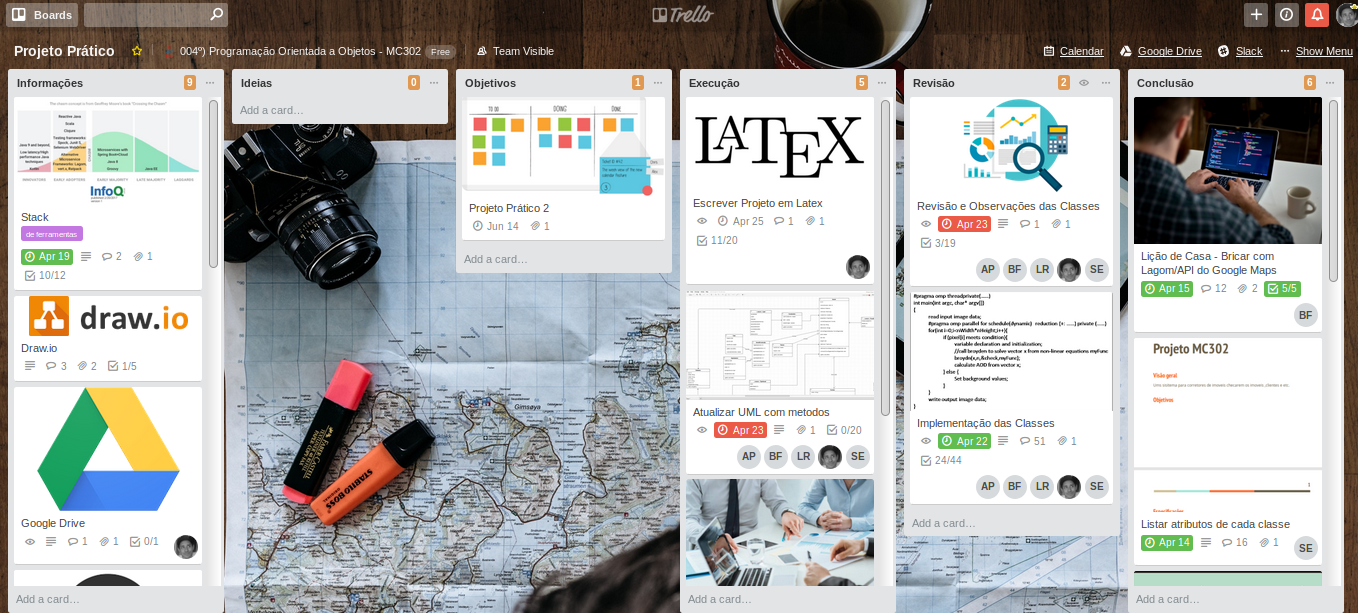
\includegraphics[scale=0.3]{imagens/trello.png}
  \end{center}
  \caption{Como o Trello é usado no nosso projeto}
  \label{f:trello}
\end{figure}

O nosso board é dividido em 6 listas: Informações, Ideias, Objetivos, Execução, Revisão e Conclusão.

Informações: Tem cards com informações gerais, links, recursos e descrições e documentações das ferramentas que estamos utilizando.

Ideias: Lista para cards de ideias gerais.

Objetivos: Lista com os objetivos futuros que estamos galgando.

Execução: Lista com as tarefas que estão sendo executadas naquela fase do projeto.

Revisão: Revisão das tarefas terminadas em Execução.

Conclusão: Tarefas que foram em grande parte feitas.

\subsection{Google Hangouts}
\label{ss:google-hangouts}

O Google Hangouts é o serviço padrão da Google para comunicação em tempo real.
  Usamos muito durante nossas reuniões remotas. Normalmente nos encontramos mais online
    do que fisicamente devido aos diferentes horários em comum entre os membros.

Conseguimos com ele compartilhamento de tela compartilhamento de áudio e essas features são as mais usadas entre
  nós.

\subsection{Google Drive}
\label{ss:google-drive}

Usamos para ter os dados mais atualizados possível de forma sincronizada. O Trello e o draw.io tem integração com o Drive que
  usamos constantemente entre nós.

\subsection{draw.io}
\label{ss:draw}

Para a criação do Diagrama de Classes UML presente neste arquivo foi utilizado o draw.io, uma ferramenta online de criação e edição de diversos tipo de diagramas.
 O site permite integração dos diagramas com o Google Drive, que é útil para compartilhamento dos diagramas e edição simultânea por mais de um membro.


\subsection{Whatsapp}
\label{ss:whatsapp}

Usado para comunicação rápida entre os membros.

\subsection{LaTeX}
\label{ss:latex}

O \LaTeX é utilizado para a formatação do nosso relatório final sobre o projeto. O arquivo lido atualmente foi compilado pelo LaTeX e
  nos proporciona vários benefícios relacionados a escrita. É uma ferramenta com grande uso pela comunidade acadêmica.

\subsection{WindowsBuilder}
\label{ss:windows-builder}

O WindowsBuilder é um plugin para Eclipse para facilitar a criação de interfaces gráficas (GUI). Nessa fase do projeto essa
  ferramenta vai nos ajudar a entregar um projeto com uma interface gráfica simples. Vamos ter a estrutura de um CRUD (mas sem banco de dados).


\bibliographystyle{plain}
\bibliography{refs}


\end{document}
